\documentclass[10pt,conference,letterpaper]{IEEEtran}

% IEEE 中文译稿；使用 XeLaTeX 编译。
\usepackage{xeCJK}
\setCJKmainfont{Noto Serif CJK SC}
\setCJKsansfont{Noto Sans CJK SC}
\setCJKmonofont{Noto Sans Mono CJK SC}
\usepackage{cite}
\usepackage{amsmath,amssymb,amsthm}
\usepackage{newtxtext,newtxmath}
\interdisplaylinepenalty=2500
\usepackage{booktabs}
\usepackage{array}
\usepackage{graphicx}
\usepackage{xcolor}
\usepackage{url}
\usepackage{microtype}
\usepackage[hidelinks]{hyperref}

\renewcommand{\arraystretch}{1.06}
\setcounter{dbltopnumber}{2}
\renewcommand{\dbltopfraction}{0.92}
\renewcommand{\textfraction}{0.05}
\setlength{\dblfloatsep}{2pt plus 1pt minus 1pt}
\makeatletter
\setlength{\@dblfptop}{0pt}
\setlength{\@dblfpsep}{6pt}
\setlength{\@dblfpbot}{0pt plus 1fil}
\makeatother
\newtheorem{proposition}{命题}
\newcommand{\method}{WLCR-SEA}
\newcommand{\routing}{结构化季节专家路由}
\newcommand{\originalmethod}{Original WLCR-LightGBM}
\newcommand{\fixedmixture}{固定季节专家混合}
% Generated by tools/sync_rq4_evidence.py; do not edit by hand.
% manifest sha256: c8f920038d1537b32e429a3fcd32f4fe4d2d4907aad28b6e92f0a69453df24ed
% summary sha256: d17ed50074eb55013c933445b7de90fc8db725a07fb88cb00ab6135f83fc8d91
% protocol sha256: 3210382dc7bcfc7d78293178c12e1b3a850297a78d77d08e15e69b1016b127e6
\newcommand{\RQFourWLCRWAPE}{0.1967}
\newcommand{\RQFourDLinearWAPE}{0.1945}
\newcommand{\RQFourDLinearDelta}{+0.00216}
\newcommand{\RQFourDLinearCILow}{-0.00124}
\newcommand{\RQFourDLinearCIHigh}{0.00636}
\newcommand{\RQFourOriginalWAPE}{0.2002}
\newcommand{\RQFourOriginalDelta}{-0.00349}
\newcommand{\RQFourOriginalCILow}{-0.00890}
\newcommand{\RQFourOriginalCIHigh}{0.00086}
\newcommand{\RQFourPatchWAPE}{0.2171}
\newcommand{\RQFourPatchDelta}{-0.02036}
\newcommand{\RQFourPatchCILow}{-0.02679}
\newcommand{\RQFourPatchCIHigh}{-0.01439}
\newcommand{\RQFourSameHourWAPE}{0.2096}
\newcommand{\RQFourFixedMixtureWAPE}{0.2368}
\newcommand{\RQFourStandardStatWAPE}{0.2270}
\newcommand{\RQFourPriorMassPercent}{1.83}
\newcommand{\RQFourClusterCount}{727}
\newcommand{\RQFourEvaluationWindowCount}{5,110}
\newcommand{\RQFourModelSeed}{42}
\newcommand{\RQFourAugmentationSeed}{100042}
\newcommand{\RQFourWLCRBatchSize}{256}
\newcommand{\RQFourNeuralBatchSize}{128}


\title{面向可审计请求局部蜂窝话务预测的结构化季节专家路由}
\author{\IEEEauthorblockN{匿名作者}
\IEEEauthorblockA{匿名机构\\匿名邮箱}}

\begin{document}
\maketitle

\begin{abstract}
部署于隔离边缘域的短期蜂窝预测服务可以共享全局模型，却被禁止读取当前目标小区请求之外的实时话务。这一请求局部约束排除了依赖实时跨小区信号的预测器，并要求预测路径能够仅凭获授权证据重现。我们提出结构化季节专家路由，并将其具体化为 WLCR-SEA。对每个 336 小时请求，WLCR-SEA 构造八个具名的季节性与汇总专家，对不可用专家实施硬掩码，通过按预测步长调节的掩码 Entmax 在可用证据上进行路由，并围绕路由基线约束学习得到的修正量。有限专家接口显式提供重放和检查每项预测所需的数值、掩码、权重和残差，而无需访问其他小区。
在来自 736 个小区、包含 527,760 条小区--小时记录的探索性 8 月评估中，WLCR-SEA 相对既有仅话务模型的 WAPE 差异为 $+0.00045$，未调整的 95\% 小区簇 bootstrap 区间为 $[-0.00312,0.00366]$；DLinear 的干净 WAPE 最低。在匹配的 15\% 缺失增强下，相对 DLinear-Aug 和 PatchTST-Aug 的六个选定中等缺失比较区间均包含零。在列出的 50\% 块缺失、时间线尾部缺失和异步缺失条件下，相对三个增强匹配基线的九个差异均为负，且未调整区间均低于零；这些结果以五个固定破坏掩码为条件。记录的实现测试得到不可用专家权重为零、有界包络违例为零，并在字段白名单下的 256 个分层请求对象测试中保持按位不变。五个种子模型组成的 CPU 集成在单线程、批量为一的协议下测得 34.70/38.68 ms 的 P50/P99 延迟。这些结果描述的是探索性的鲁棒性--可检查性--成本剖面，而非普适优势。
WLCR-SEA 的可复现源码已随本文开源发布。
\end{abstract}

\begin{IEEEkeywords}
蜂窝话务预测，请求局部推理，结构化专家路由，稀疏注意力，遥测缺失，可审计性
\end{IEEEkeywords}

\section{引言}
短时蜂窝话务预测支持前瞻性的无线资源与服务容量规划。设想一个蜂窝网络：其运行策略只允许预测服务读取待预测小区的实时话务。对每个任务，服务接收一个 336 小时历史窗口及其观测掩码，并且必须仅据此生成 24 小时预测。我们将其称为请求局部服务。部署时，身份感知的前端服务（即入口）授权请求，并将该窗口封装为密封的、自包含输入\footnote{入口可使用小区标识符进行授权和路由；评分器既不将其作为模型特征接收，也不利用它发起按身份条件化的查询。}；评分器再将其与预置的全局检查点结合，后者是由所有请求共享且带版本的模型。这样的安排在自适应预测与能够仅凭该请求获授权的证据重现的预测路径之间形成张力。

我们的核心洞见是，蜂窝话务预测可分解为一小组具名的季节参考：前一天、上周、两周前、稳健中位数、趋势估计和先验。每个参考在给定请求中要么可用，要么不可用。与其让黑盒模型隐式推断哪些参考重要，我们显式构造这些候选，对不可用者实施硬掩码，并只学习随预测步长和上下文变化的混合权重以及有界修正。我们将该设计具体化为 \method{}，即窗口局部上下文表征与季节专家注意力。

\begin{figure}[t]
\centering
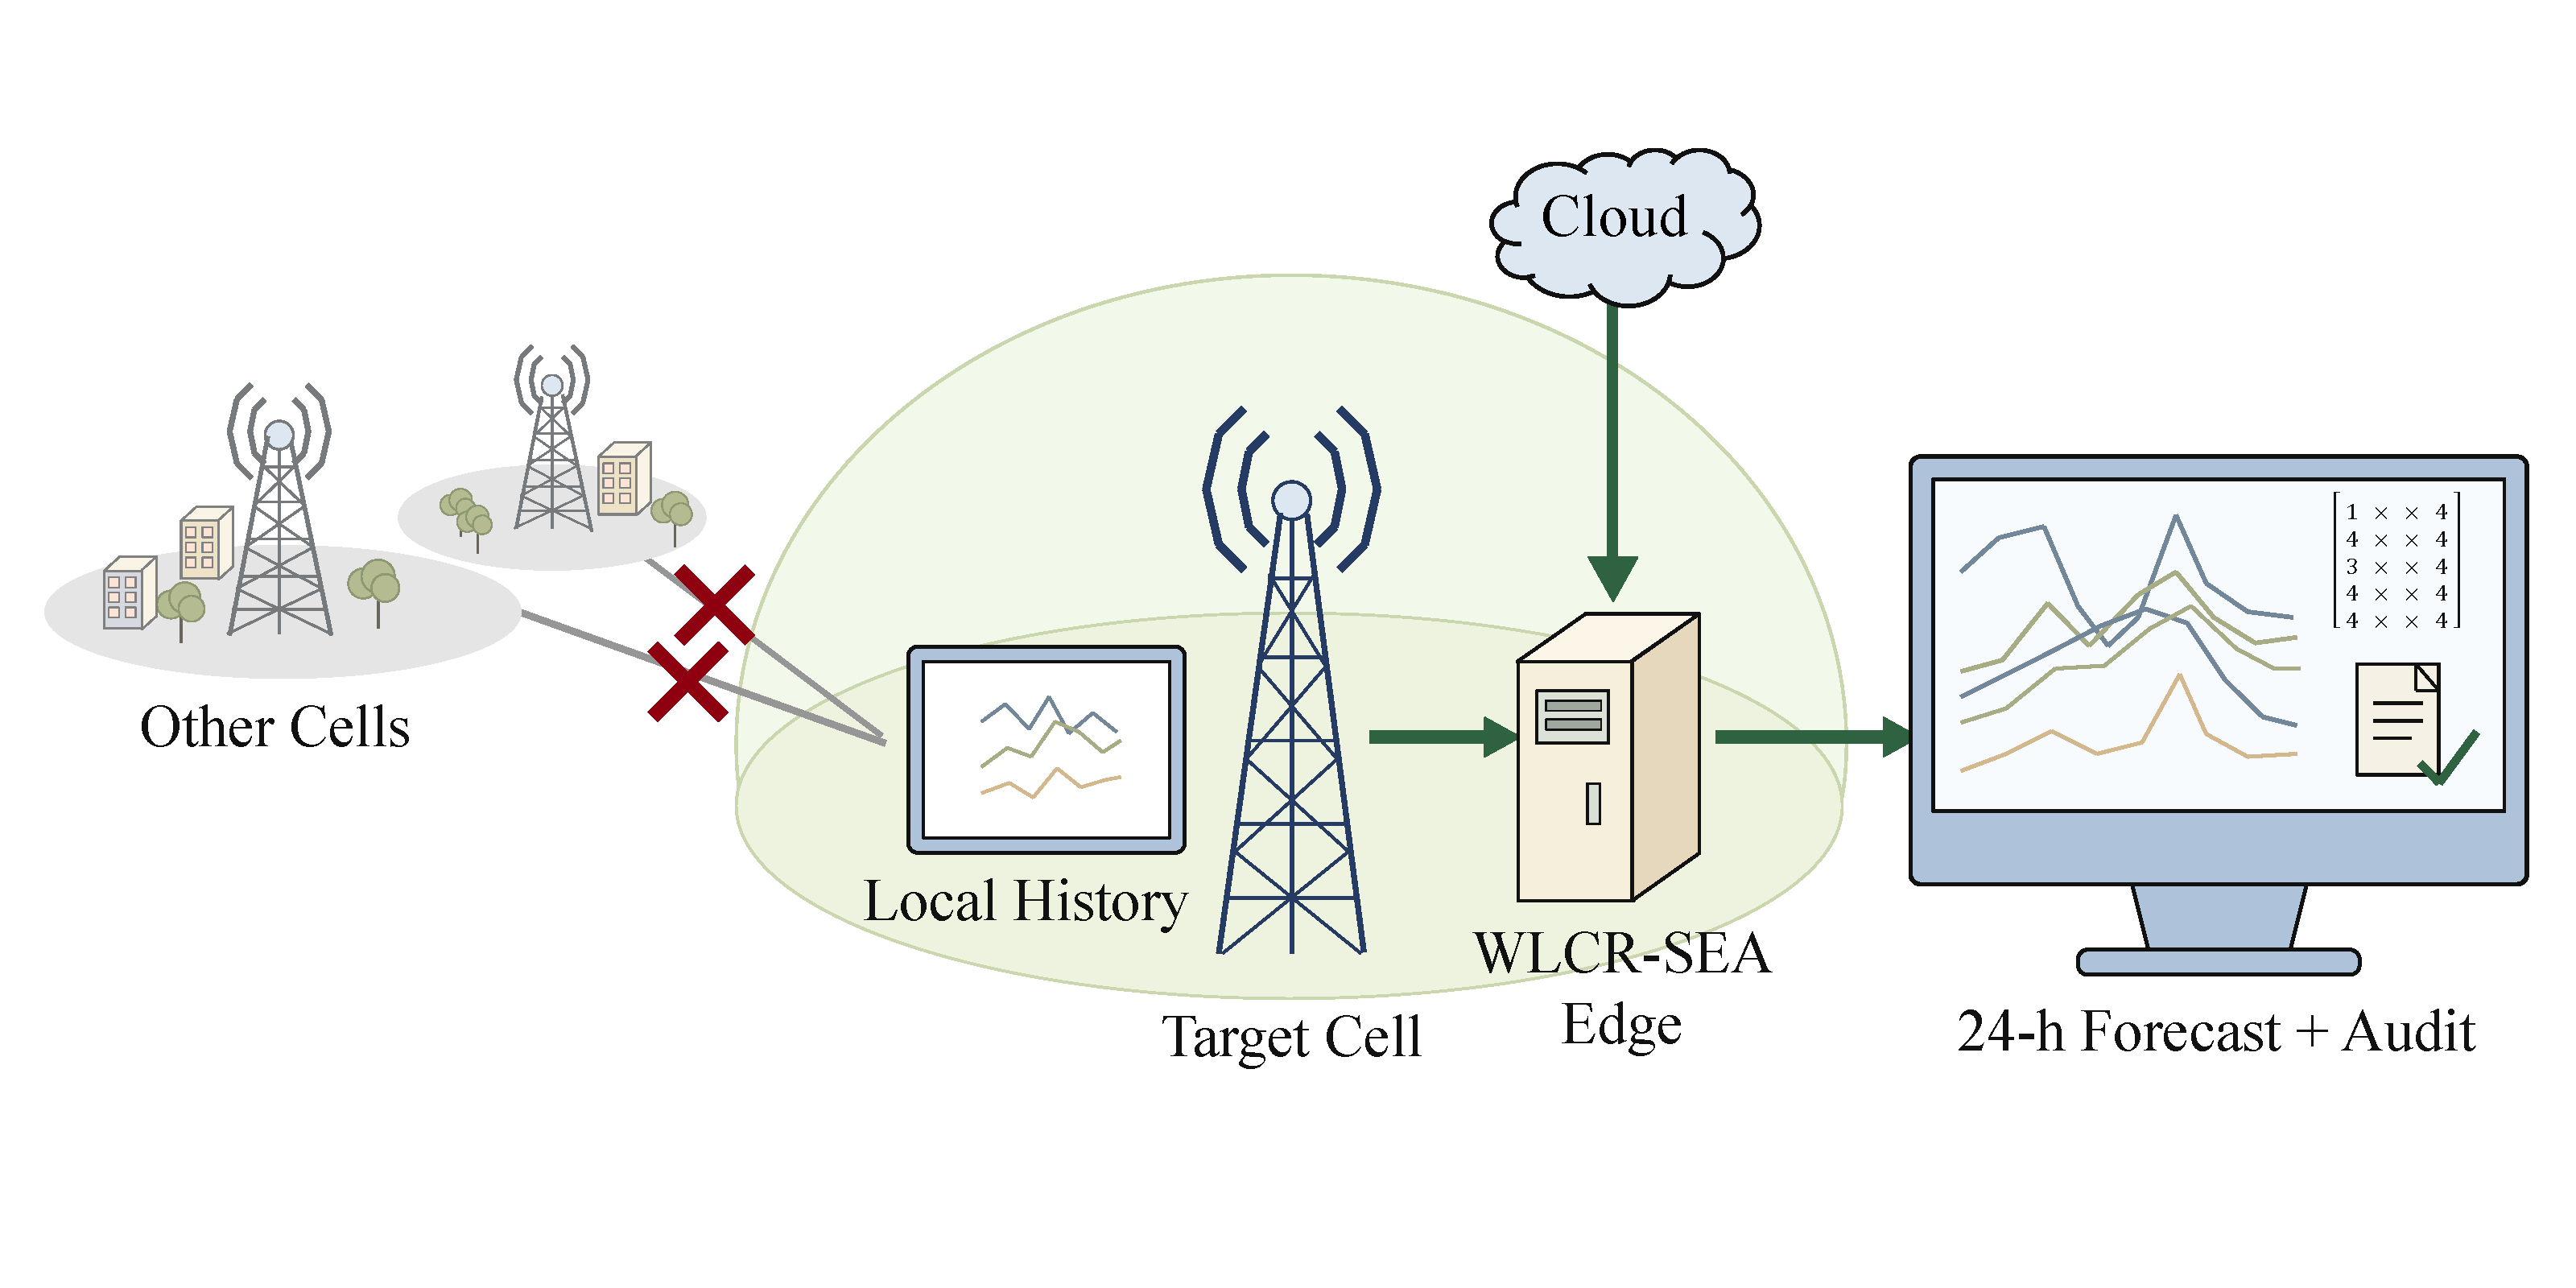
\includegraphics[width=\columnwidth,trim={80pt 70pt 180pt 50pt},clip]{figures/Scene_Diagram.pdf}
\caption{概念性请求局部服务场景。入口可利用运行身份授权并生成一个密封请求，预测进程则接收该请求和预置检查点。该场景界定了一条自包含的在线评分路径及其可审计的证据边界。}
\label{fig:scenario}
\end{figure}

本文贡献如下：
\begin{itemize}
\item 我们形式化请求局部服务策略，并验证其实现服务路径的请求对象不变性。
\item 我们基于八个具名专家开发\routing{}，采用预测步长和上下文条件化分配、严格可用性掩码及有界残差。
\item 我们评估干净数据精度、增强匹配的缺失鲁棒性、小区不相交重拟合、审计属性和同机延迟。
\end{itemize}

本文不主张普适预测优势或等效性；我们评估的是上述服务策略下探索性的鲁棒性--可检查性--成本剖面。


\section{相关工作}
\textbf{时空蜂窝话务预测。}
蜂窝话务具有时间与空间结构，因而催生了循环、卷积、注意力和图模型~\cite{huang2017study,zhang2018long,wang2019spatiotemporal,zhao2022aggregation,wang2022attention,yao2023mvstgn,mehrabian2023bernstein}。图和多小区方法利用拓扑和邻居话务来捕捉空间依赖。这些方法假定评分时可以访问跨小区信号，而 WLCR-SEA 从一个密封的目标请求生成预测。

\textbf{请求局部服务。}
联邦学习在共享模型更新的同时限制原始数据的集中收集~\cite{zhang2021dualattention}。本文关注的问题则是：身份感知的入口生成密封输入并预置共享检查点后，一个评分请求能够读取何种证据。这一部署视角以请求局部证据而非去中心化训练作为核心差异。

\textbf{有限历史与不完整输入下的预测。}
全局模型可在预测时不读取其他序列的情况下，学习相关序列间共享的参数~\cite{montero2021global}。DLinear 和 PatchTST 提供了强有力的分解式与分块式基线~\cite{zeng2023dlinear,nie2023patchtst}，GRU-D、SAITS 与 CSDI 则显式建模不完整时间序列~\cite{che2018grud,du2023saits,tashiro2021csdi}。GRIN 等基于图的插补还会利用序列间结构~\cite{cini2022grin}，这超出本文研究的请求局部服务策略。预测组合和动态模型平均也用于处理大规模、随时间变化的预测问题~\cite{makridakis2022m5,koop2012forecasting}。不同于这些预测器，WLCR-SEA 为每次预测公开由具名参考、可用性掩码、分配权重、基线和残差组成的有限接口。

\textbf{稀疏专家路由。}
稀疏专家混合层在学习得到的子网络之间分配计算~\cite{shazeer2017moe}，Entmax 则产生包含严格零值的归一化分配~\cite{peters2019sparse}。常规混合模型选择潜在子网络；WLCR-SEA 在具有可追溯请求索引和硬可用性掩码的具名季节估计器之间路由。因此，每个非零分配均对应一种可见的证据类型，而非潜在专家。

\section{问题表述与服务访问策略}
设 $x_{c,u,q}\geq0$ 表示小区 $c$ 在时刻 $u$、指标 $q\in\{1,\ldots,4\}$ 上的原始小时话务。按上述顺序，四项指标为平均上行活跃用户数、平均下行活跃用户数、平均下行已用物理资源块（PRB）数和平均上行已用 PRB 数；PRB 字段是已用 PRB 的平均计数而非利用率。观测掩码为 $m_{c,u,q}\in\{0,1\}$。在小时 $t$ 结束的一个请求包含
\begin{equation}
\mathcal W_{c,t}=\{(\bar{\mathbf x}_{c,u},\mathbf m_{c,u})\}_{u=t-335}^{t},
\end{equation}
其中，对于观测值有 $\bar x=\log(1+x)$。缺失位置的数值填充仅用于数值计算，不具有语义上的权威性，因为每一步操作都同时接收 $m$。目标是同四条序列的下一段：
\begin{equation}
\mathbf y_{c,t+h}=\mathbf x_{c,t+h},\qquad h=1,\ldots,24.
\end{equation}

所有评估请求均从午夜开始。我们将 $t$ 定义为最后一个观测到的 23:00 小时，故 $h=1$ 是紧随其后的 00:00 目标。相隔 $d$ 天的季节参考使用如下历史索引
\begin{equation}
i(h,d)=335+h-24d.
\end{equation}
当 $h\in[1,24]$ 且 $d\in[1,14]$ 时，$i(h,d)\in[0,335]$，从而消除午夜边界可能出现的小时偏移歧义。

全局拟合得到的预测器 $F_{\Theta}$ 必须满足
\begin{equation}
\widehat{\mathbf y}_{c,t+1:t+24}=F_{\Theta}(\mathcal W_{c,t})
\end{equation}
其前提是上游系统已生成 $\mathcal W_{c,t}$。符号 $c$ 在表述中标记请求来源；它不作为特征或查询键传入 $F_{\Theta}$。预测时，$F_{\Theta}$ 不得查询 $c'\neq c$ 的话务、小区专属元数据文件、拓扑或邻居表、外部特征存储或跨请求话务缓存。允许冻结训练统计量和全局共享检查点参数 $\Theta$，因为它们是对全部请求通用的预置、版本化资产，而非由目标条件决定的查询。不透明的请求/来源标识符可保留在 $F_{\Theta}$ 之外用于授权与审计。

\begin{proposition}[请求对象服务路径不变性]
在检查点参数、冻结训练先验、确定性预处理、软件状态和浮点执行模式固定时，包含相同目标对象的两个预提取请求对象集合，无论其非目标请求对象如何，均产生完全相同的专家张量、路由权重、残差和预测。
\end{proposition}
\begin{proof}
实现中的推理字段白名单仅含目标请求的\textit{x\_values}、\textit{x\_masks}、冻结先验和全局共享检查点参数；其中既无小区标识符，也无能够执行基于身份查询的客户端代码。在所述执行条件下，后续每个张量均是这些输入的确定性组合。
\end{proof}

\section{结构化季节专家路由}
\subsection{有限季节专家库}
为简洁起见，令 $z_{u,q}=\log(1+x_{c,u,q})$。表~\ref{tab:experts} 针对每个预测步长 $h$ 和指标 $q$ 定义八个专家。中位数仅使用观测值。先验
\begin{equation}
\mu^{\mathrm{train}}_{h,q}=
\operatorname{median}_{(c,t)\in\mathcal T,\;m_{c,t+h,q}=1}
\log(1+y_{c,t+h,q})
\end{equation}
仅由当前适用训练层估计，并存储为冻结的 $24\times4$ 参数。

选择这八个专家的依据如下。蜂窝话务主要受日周期和周周期支配。专家 1--3 捕捉三种季节性滞后；专家 4--5 提供稳健的同小时汇总；专家 6 编码有界的周趋势；专家 7 是退化情形下的回退；专家 8 始终可用。它们覆盖了人工预测者会检查的证据类型，使路由分配可作为模型内部行为直接检查，但其本身并非因果解释。

\noindent\textbf{示例。} 设指标 $q=1$ 的目标时刻 $t+h$ 为星期二下午 2 点。专家 1 读取星期一下午 2 点的观测话务，专家 2 读取此前一个星期二下午 2 点的值，专家 4 则对此前七天中可用的下午 2 点值取中位数。若此前一个星期二的值缺失（$m_2=0$），专家 2 会被硬掩码：任何先验填充仅为数值占位，其路由权重严格为零，路由器无法通过学习到的分配将其恢复。

\begin{table*}[t]
\centering
\caption{有限专家库。log1p 域中 $\kappa=0.5$。不可用值仅为保证张量计算安全而由先验进行数值填充；其掩码仍为零，硬路由器不会为其分配权重。}
\label{tab:experts}
\footnotesize
\setlength{\tabcolsep}{4.0pt}
\begin{tabular}{c>{\raggedright\arraybackslash}p{0.19\textwidth}>{\raggedright\arraybackslash}p{0.34\textwidth}>{\raggedright\arraybackslash}p{0.30\textwidth}}
\toprule
$j$ & 专家 & 对数域数值 $v^{(j)}_{h,q}$ & 可用性与可靠性 $\rho_j$\\
\midrule
1 & 前一天 & $z_{t+h-24,q}$ & 已观测点；$\rho_1=1$\\
2 & 前一周 & $z_{t+h-168,q}$ & 已观测点；$\rho_2=1$\\
3 & 两周滞后 & $z_{t+h-336,q}$ & 已观测点；$\rho_3=1$\\
4 & 同小时中位数，7 天 & $\operatorname{median}_{d=1}^{7}z_{t+h-24d,q}$ & 至少一个值；观测计数$/7$\\
5 & 同小时中位数，14 天 & $\operatorname{median}_{d=1}^{14}z_{t+h-24d,q}$ & 至少一个值；观测计数$/14$\\
6 & 有界周趋势 & $v^{(2)}+\operatorname{clip}(v^{(2)}-v^{(3)},-\kappa,\kappa)$ & 专家 2 和 3 已观测；取最小可靠性\\
7 & 窗口局部中位数 & $\operatorname{median}_{u=t-335}^{t}z_{u,q}$ & 任一观测值；观测计数$/336$\\
8 & 冻结训练先验 & $\mu^{\mathrm{train}}_{h,q}$ & 始终可用；$\rho_8=1$\\
\bottomrule
\end{tabular}
\end{table*}

归一化的\emph{名义新近性描述符}为
\begin{equation}
\boldsymbol\Delta=(24,168,336,96,180,252,168,0)/336.
\end{equation}
它是在完整数据下固定的专家类型描述符，而不是请求特定缺失后的实际平均证据年龄。先验中的零值是与专家类型绑定的哨兵值，并不表示近期请求证据。

目标指标上下文为
\begin{equation}
\mathbf s_{c,t,q}=[\operatorname{mean},\operatorname{median},\operatorname{sd},
r_{\mathrm{miss}},r_{\mathrm{trend}}],
\end{equation}
其由请求内观测到的对数值计算得到。仅有一个观测时标准差为零。趋势定义为
\begin{equation}
r_{\mathrm{trend}}=
\operatorname{median}(z_{t-23:t,q})-
\operatorname{median}(z_{t-47:t-24,q}),
\end{equation}
其使用观测值计算；若任一整天没有观测，则设为零。

\subsection{预测步长条件化稀疏路由器}
对 A1--A3，专家 $j$ 的表征不含可靠性，
\begin{equation}
\mathbf e^{\mathrm{A1:A3}}_j=[\mathbf e^{\mathrm{type}}_j,v_j,m_j,\Delta_j],
\end{equation}
而 A4--A6 使用
\begin{equation}
\mathbf e^{\mathrm{A4:A6}}_j=[\mathbf e^{\mathrm{type}}_j,v_j,m_j,\Delta_j,\rho_j].
\end{equation}
查询向量为 $\mathbf q_{h,q}=g_Q([\mathbf e_h,\mathbf e_q,\mathbf s_{c,t,q}])$。对 A4--A6，评分还包含可靠性偏置，
\begin{equation}
\begin{aligned}
a_j&=\frac{\mathbf q_{h,q}^{\top}g_K(\mathbf e_j)}{\sqrt d}
+\beta\log\!\left(\max\{\rho_j,10^{-6}\}\right),\\
\beta&=\operatorname{softplus}(\widetilde\beta),
\end{aligned}
\end{equation}
该偏置和 $\mathcal L_{\mathrm{rel}}$ 在 A1--A3 中均不使用。

对每个硬掩码路由器，令 $\mathcal J=\{j:m_j=1\}$。分配定义在可用集合上：
\begin{align}
\boldsymbol\alpha_{\mathcal J}
 &=\operatorname{Entmax}_{1.5}(\{a_j:j\in\mathcal J\}),\\
\alpha_j&=0,\qquad j\notin\mathcal J .
\end{align}
实现将每个可用子集压紧，在该子集上施加 Entmax，再将结果散射回八专家轴；它不以有限负分数充当排除替代。因此，不可用专家在结构上具有严格为零的分配权重。在 A1 和 A2 中，不可用专家保留其先验填充值与可用性标记 $m_j=0$，但路由仍在全部八个 logit 上计算，可能为其分配非零权重。A2 中的 Entmax 可能产生稀疏分配，却无法从结构上保证不可用专家权重为零；A3 以结构性排除取代该学习响应。

学习得到的静态对照采用同一可用集合约定：
\begin{align}
\boldsymbol\alpha_{q,\mathcal J}&=\operatorname{softmax}(\{\theta_{q,j}:j\in\mathcal J\}), &&32\text{ parameters},\\
\boldsymbol\alpha_{h,q,\mathcal J}&=\operatorname{softmax}(\{\theta_{h,q,j}:j\in\mathcal J\}), &&768\text{ parameters},
\end{align}
在 $\mathcal J$ 外权重为零。\emph{\fixedmixture{}} 使用权重 $(0,0.7,0.2,0.1,0,0,0,0)$，移除不可用专家后重新归一化；若剩余固定权重为零，则回退至先验。该确定性基线不同于 \originalmethod{}。

\begin{table}[t]
\centering
\caption{路由器变体。可靠性模块包括可用性标记、评分偏置和辅助损失。在本消融表之外，\method{} 指代变体 A6。}
\label{tab:variants}
\footnotesize
\setlength{\tabcolsep}{2.0pt}
\renewcommand{\arraystretch}{1.05}
\begin{tabular*}{\columnwidth}{@{\extracolsep{\fill}}clcccc@{}}
\toprule
编号 & 路由器 & \shortstack{硬\\掩码} & 可靠性 & \shortstack{有界\\残差} & \shortstack{混合 15\%\\增强}\\
\midrule
A1 & Softmax & 否 & 否 & 否 & 否\\
A2 & Entmax$_{1.5}$ & 否 & 否 & 否 & 否\\
A3 & Entmax$_{1.5}$ & 是 & 否 & 否 & 否\\
A4 & Entmax$_{1.5}$ & 是 & 是 & 否 & 否\\
A5 & Entmax$_{1.5}$ & 是 & 是 & 是 & 否\\
A6 & Entmax$_{1.5}$ & 是 & 是 & 是 & 是\\
\bottomrule
\end{tabular*}
\end{table}

\subsection{有界潜在审计包络}
动态基线与熵为
\begin{align}
b_{c,t,h,q}&=\sum_{j=1}^{8}\alpha_{c,t,h,q,j}v^{(j)}_{c,t,h,q},\\
H(\boldsymbol\alpha)&=-\sum_j\alpha_j\log(\alpha_j+10^{-12}).
\end{align}
一个小型网络接收 $b$、局部上下文、预测步长和指标嵌入以及 $H$，并产生
\begin{align}
\delta&=\delta_{\max}\tanh g_R(b,\mathbf s,\mathbf e_h,\mathbf e_q,H),\\
\widehat\ell&=b+\delta,\qquad
\widehat y=\max\{10^{-4},\exp(\widehat\ell)-1\}.
\end{align}
候选边界在未归一化 log1p 单位中为 $\delta_{\max}\in\{0.25,0.5\}$，并在内层数据上选择。凸组合变体令 $\delta_{\max}=0$。

\begin{proposition}[有界潜在审计包络]
令 $\mathcal J=\{j:m_j=1\}$。由于先验始终可用，应用输出下限前的潜在预测满足
\begin{equation}
\min_{j\in\mathcal J}v_j-\delta_{\max}
\leq \widehat\ell \leq
\max_{j\in\mathcal J}v_j+\delta_{\max}.
\end{equation}
因此，最终原始尺度预测落在
\begin{equation}
\left[\max\{10^{-4},e^{v_{\min}-\delta_{\max}}-1\},
\max\{10^{-4},e^{v_{\max}+\delta_{\max}}-1\}\right],
\end{equation}
其中 $v_{\min}$ 和 $v_{\max}$ 分别是 $\mathcal J$ 上的最小值和最大值。
\end{proposition}
\begin{proof}
对硬掩码变体，动态基线是可用专家值的凸组合，因而位于其凸包中。加入绝对值不超过 $\delta_{\max}$ 的残差即可得到潜在边界；指数函数的单调性和最终非负下限给出原始域区间。
\end{proof}

\subsection{训练、增强与请求记录}
WLCR-SEA 将专家值、先验、残差和掩码 L1 目标均定义在\emph{未归一化} log1p 域中。对观测目标，它最小化
\begin{equation}
\mathcal L=\mathcal L_{\mathrm{pred}}
+10^{-3}\mathcal L_{\mathrm{res}}
+\lambda_{\mathrm{rel}}\mathcal L_{\mathrm{rel}},
\end{equation}
其中 $\mathcal L_{\mathrm{pred}}$ 是未归一化 log1p 预测与目标间的掩码 L1，$\mathcal L_{\mathrm{res}}=\operatorname{mean}(\delta^2)$，而 $\mathcal L_{\mathrm{rel}}=\operatorname{mean}_j[\alpha_j(1-\rho_j)]$。仅对 A4--A6 设置 $\lambda_{\mathrm{rel}}=10^{-3}$，对 A1--A3 则严格设为零。

对 \method{}（A6），在每个拟合或最终训练阶段以及每个数据/模型种子下，均确定一个固定的 15\% 输入历史视图，并在所有 epoch 中保持不变。稳定哈希为每个小区均匀选择 MCAR、块缺失、时间线尾部缺失或异步缺失之一。MCAR、块缺失和时间线尾部掩码跨指标同步；异步掩码按指标独立。掩码在窗口提取前按唯一小区--时间键生成，再投影到重叠请求中；标签和目标掩码不变。为公平比较鲁棒性，\method{}、DLinear-Aug、PatchTST-Aug 和 GRU-D-Direct-Aug 以相同数据种子调用同一确定性掩码生成器，因而接收相同的预生成视图；最终阶段对模型种子 $s$ 使用种子 $s+100000$。

服务计算会输出拟议的固定模式语义审计记录的核心字段：
\begin{equation}
\mathcal A_{c,t,h,q}=
\{\alpha_j,v_j,m_j,\rho_j\}_{j=1}^{8}
\cup\{b,\delta,H,|\operatorname{supp}(\alpha)|\}.
\end{equation}
部署记录还包含模式标识、检查点哈希和变换版本标识；其序列化不包含在报告的延迟基准中。图~\ref{fig:architecture} 概述请求路径。

\begin{figure*}[t]
\centering
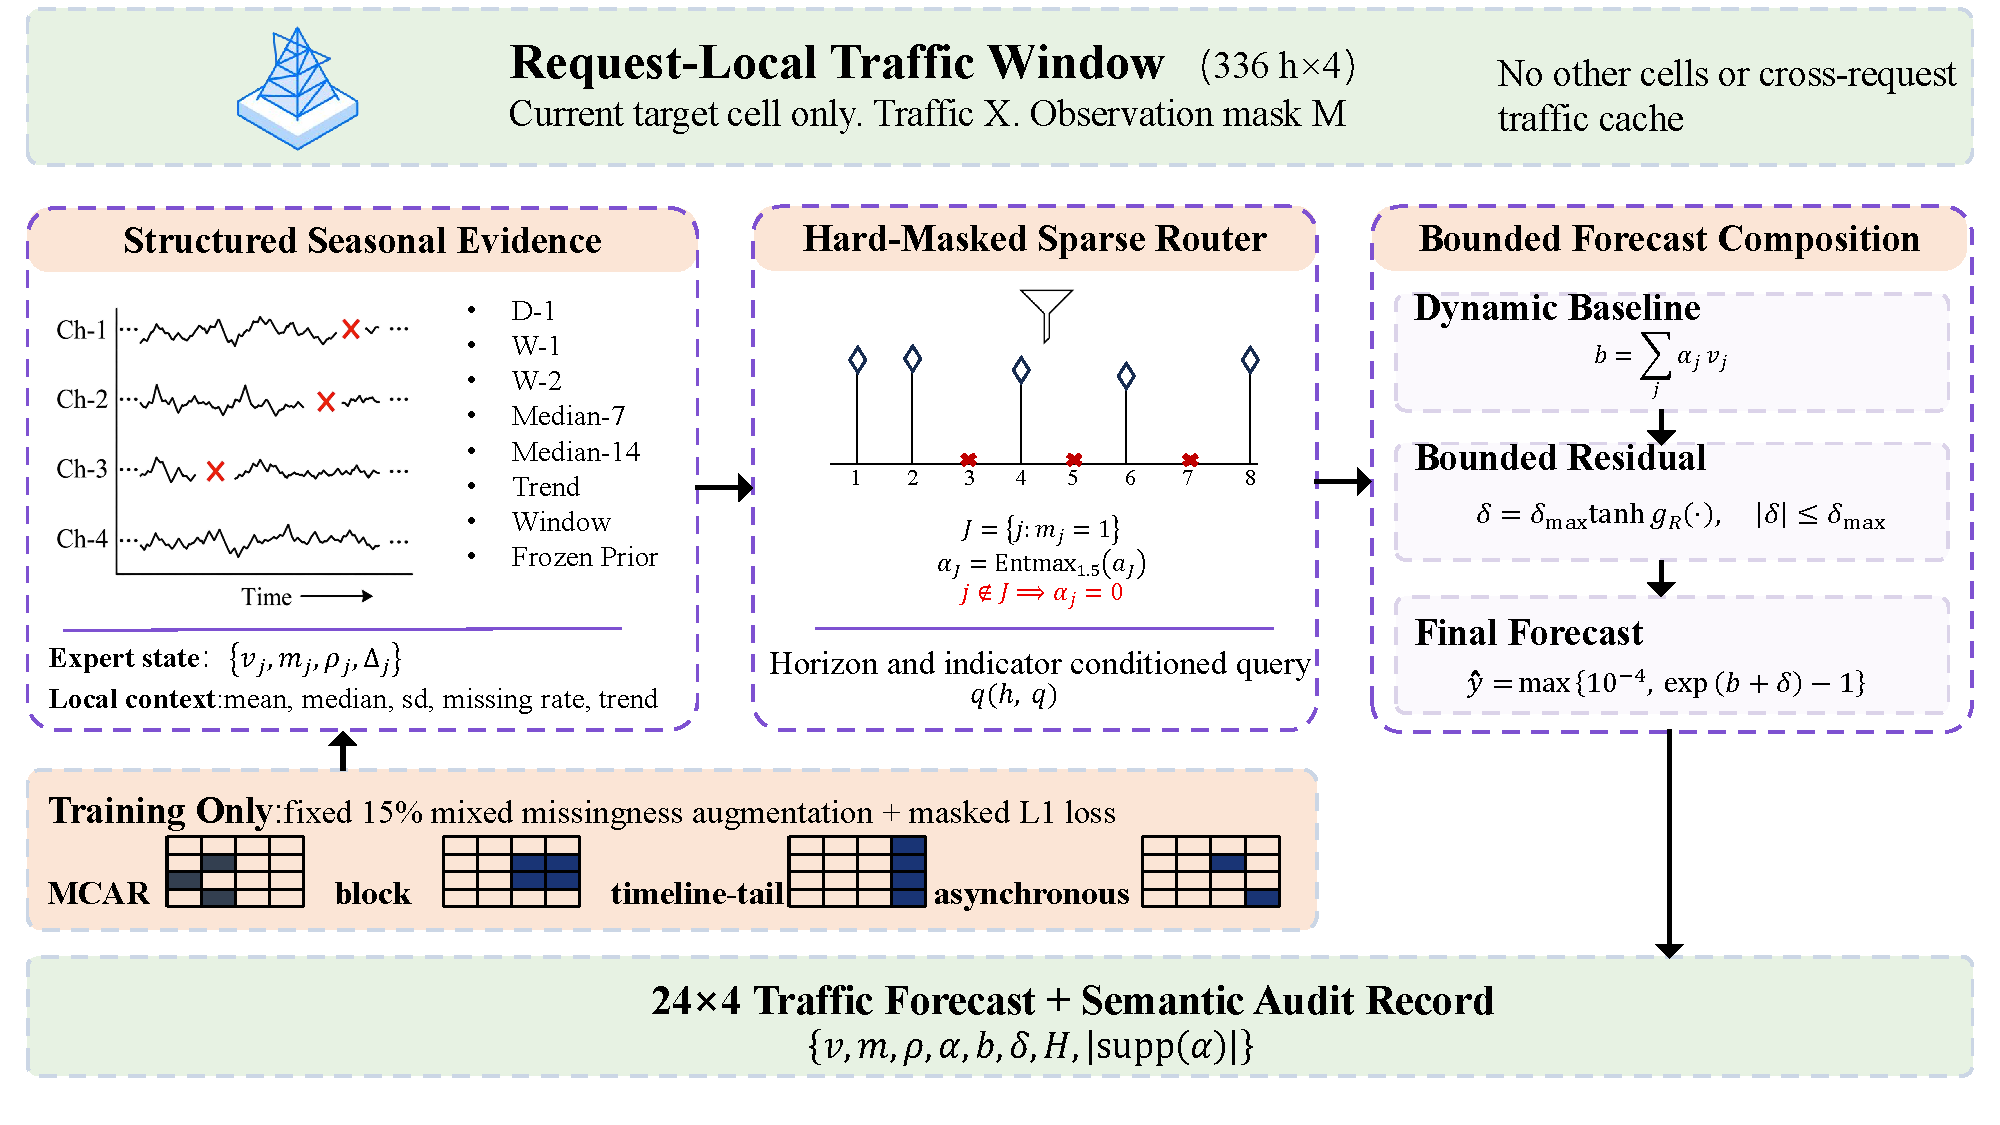
\includegraphics[width=\textwidth]{figures/fig_architecture.pdf}
\caption{作为结构化季节专家路由实例的 \method{}。一个掩码 336 小时请求构造有限专家库；预测步长条件化路由对不可用证据实施硬掩码，并产生动态基线、有界修正、$24\times4$ 预测和拟议审计记录的核心字段。}
\label{fig:architecture}
\end{figure*}

\section{实验方法}
\subsection{数据、划分与证据状态}
匿名轨迹包含 2024 年 7 月 20 日至 8 月 18 日间、来自 736 个小区的 527,760 条小时记录。该面板并非完整面板：730 个小区各含 720 小时，6 个各含 360 小时。每项指标均有 69,014 个缺失小区--小时值，即 527,760 条小区--小时记录的 13.08\%；四项指标共享观测掩码。

按日滑动产生 11,686 个候选窗口，每个窗口包含 336 小时输入和 24 小时预测。其中一个窗口（小区 2062，起点为 8 月 4 日）存在 25 小时的不连续性，因而被报告而非修复；其余为 11,685 个连续窗口。8 月 3--9 日目标构成拟合层（5,115 个窗口），8 月 10--11 日构成内层（1,460 个），8 月 12--18 日构成评估层（5,110 个）。全部 730 个长序列小区各贡献七个评估窗口。727 个小区定义了按小区 WAPE；另三个在目标掩码后缺少正的可评估分母。评估包含 122,640 个预测小时及每项指标 106,248 个观测目标小时。

该评估期已在研究早期迭代阶段使用过。对于后续 GRU-D 比较，其候选网格、内层选择规则、增强视图、五个模型种子（42--46）、破坏种子（142--146）、指标和 bootstrap 程序均在比较执行及最终汇总前预先固定。这些选择确保该比较在执行和最终汇总中遵循固定协议。

\subsection{基线、公平性与优化}
干净比较包括同小时中位数、\fixedmixture{}、学习得到的全局与步长--指标混合、165 维 Standard-stat LightGBM、精确对齐的仅话务 \originalmethod{}、DLinear、PatchTST、GRU-D-Direct-Aug 以及 A1--A6 路由器变体。\originalmethod{} 的精确对齐覆盖全部 122,640 个预测键且无重复。两个树模型基线均采用 LightGBM~\cite{ke2017lightgbm}，参数为 48 个叶节点、最小叶节点大小 80、学习率 0.04、特征采样比例 0.88、bagging 比例 0.90、$\lambda_1=0.05$、$\lambda_2=0.20$ 和最大 bin 数 127。\originalmethod{} 使用 73 个仅话务特征及固定的目标专属迭代轮数 341/332/742/678。

主要鲁棒性分析采用受控的增强匹配比较，将 \method{}（A6）与 DLinear-Aug、PatchTST-Aug 和适配后的缺失感知 GRU-D-Direct-Aug 对照进行比较。对五个模型种子中的每一个，四个模型均接收同一确定性 15\% 混合输入历史视图，并使用相同的拟合日期、内层日期及拟合加内层重拟合流程。选择均仅在同一内层日期上进行，但准则因模型族而异：WLCR-SEA 最小化指标间宏平均 WAPE，并以由拟合层冻结的 THS 打破平局；神经基线则最大化代码中记为 MAPEAUC 的四个 MAPE 命中率均值，该指标采用由内层自身得到的第五百分位筛选，并以更低的内层平均 MAPE 打破平局。以干净数据训练的 DLinear 和 PatchTST 仅用于量化增强的独立贡献。

DLinear、PatchTST 和 GRU-D-Direct-Aug 使用当前适用训练层的统计量归一化 log1p 输入和目标：候选选择阶段使用拟合日期，最终重拟合阶段使用拟合加内层日期；它们在\emph{归一化目标空间}最小化掩码 L1，并在原始尺度评估前将预测反归一化。GRU-D-Direct-Aug 严格在每个 336 小时请求内计算缺失扰动后各指标的时间间隔：在请求的首小时，若该指标有观测则 $\Delta_{1,q}=0$，否则 $\Delta_{1,q}=1$。若该请求内不存在更早观测，则其前值初始化为当前适用训练层的均值（标准化空间中为零）；不查询窗口前遥测。模型学习输入和隐藏状态衰减，将 $[\mathrm{imputed\ value},\mathrm{mask}]$ 输入 GRUCell，并将最终隐藏状态直接映射为 $24\times4$ 归一化对数预测。Dropout 0.10 仅在训练时、直接输出头之前施加于该最终隐藏状态；不使用输入或循环 Dropout。

相较之下，WLCR-SEA 对专家、先验、残差和掩码 L1 均使用未归一化 log1p 域，从而保持 $\kappa$、$\delta_{\max}$ 和审计包络的固定解释。所有神经与路由模型均使用 AdamW、权重衰减 $10^{-4}$、最多 100 个 epoch、早停耐心轮数 10 及五个模型种子。WLCR-SEA 的批量大小为 256，而 DLinear、PatchTST 和 GRU-D-Direct-Aug 的批量大小为 128。DLinear 候选为核大小 25、学习率 $10^{-3}$，及核大小 49、学习率 $5\times10^{-4}$。PatchTST 使用长度 24、步幅 12 的 patch；其候选为相应学习率下的 $(d,\mathrm{heads},\mathrm{layers},\mathrm{FF},\mathrm{dropout})=(32,4,1,64,0.1)$ 与 $(48,4,2,96,0.1)$。GRU-D-Direct-Aug 候选为学习率 $10^{-3}$ 的隐藏维度 32 和学习率 $5\times10^{-4}$ 的隐藏维度 48，二者均使用所述输出头 Dropout。路由器候选为 $(d,\mathrm{hidden},\eta,\delta_{\max})=(16,32,10^{-3},0.25)$ 或 $(32,64,5\times10^{-4},0.5)$。每个模型均使用上述模型族专属准则，仅在内层日期上选择配置和 epoch 数，随后重新初始化并在拟合加内层日期上重拟合。

对五个最终 GRU-D 成员，内层为种子 42/43/45 分别在 epoch 53/41/17 选择隐藏维度 32，为种子 44/46 分别在 epoch 95/35 选择隐藏维度 48。因此选定的最佳 epoch 范围为 17--95。种子 44 的维度 48 候选跑至 100 epoch 上限，但其选定 epoch 为 95。

我们报告五个确定性小区不相交折，作为补充性的单模型种子（42）重拟合审计，而非五个种子模型集成。对每个神经或路由模型，架构、选定配置、epoch 数和优化器设置均由其时间实验的种子 42 运行冻结。每一折都使用增强种子 100042 生成的匹配最终重拟合输入历史视图；WLCR-SEA 保持批量大小 256，DLinear-Aug 和 PatchTST-Aug 保持批量大小 128。每个外折仅在互补小区上重拟合，且不进行折特异再调优；每个评估小区均被排除在先验、归一化、神经权重、路由器权重和 booster 之外。

\subsection{指标、集成与不确定性}
全部报告的 WAPE、MASE 和 sMAPE 均在原始话务尺度反变换后计算。主要指标是指标间宏平均 WAPE：
\begin{equation}
\operatorname{WAPE}_{\mathrm{macro}}=
\frac14\sum_{q=1}^{4}
\frac{\sum_i|y_{i,q}-\widehat y_{i,q}|}{\sum_i|y_{i,q}|}.
\end{equation}
对于请求 $i$ 和指标 $q$，请求局部的 168 小时 MASE 尺度为
\begin{equation}
d_{i,q}=\frac{1}{|\mathcal P_{i,q}|}\sum_{u\in\mathcal P_{i,q}}
|x_{i,u,q}-x_{i,u-168,q}|,
\end{equation}
其中 $\mathcal P_{i,q}$ 仅保留有限的历史端点对。仅当 $\mathcal P_{i,q}$ 非空且 $d_{i,q}>10^{-12}$ 时，一个请求--指标组合才计入 MASE；MASE 对由此得到的尺度化绝对误差取平均。全部 20,356 个具有观测留出目标的请求--指标组合（424,992 个目标值）均符合 MASE 资格，故测得覆盖率为 100\%。我们将 sMAPE 定义为
\begin{equation}
\operatorname{sMAPE}=\frac{2|y-\widehat y|}{\max(|y|+|\widehat y|,10^{-12})}.
\end{equation}
此外，我们报告汇总 WAPE 和阈值命中分数（THS）。THS 在应用由当前适用训练层冻结的第五百分位筛选后，计算 MAPE 阈值 $\{0.2,0.3,0.4,0.5\}$ 下的严格命中率均值。WLCR-SEA 内层选择使用拟合日期确定筛选阈值；报告的时间留出指标使用拟合加内层日期；每个小区不相交折则使用其互补训练小区。THS 不是曲线下面积。

除非明确标记为确定性、树模型或单成员部署结果，全部主要\emph{时间}神经与路由准确性结果均采用五个种子模型的算术预测集成。小区不相交审计单独报告，并固定一个模型种子（42）。部署表另行报告每个计时的单成员或集成配置。令模型种子 $s\in\{42,\ldots,46\}$、破坏种子 $r\in\{142,\ldots,146\}$，则
\begin{equation}
\widehat y^{(r)}=\frac15\sum_s\widehat y^{(s,r)},\qquad
\bar W=\frac15\sum_r\operatorname{WAPE}(\widehat y^{(r)}).
\end{equation}
成对 95\% 区间使用 5,000 次小区簇 bootstrap 重复。每次重复重采样小区，保留每个被采样小区的全部日期和预测步长，重新计算指标专属的比值之和，再对四项指标 WAPE 取平均。对破坏结果，在每次 bootstrap 重复内先对破坏种子平均成对差异。主要成对比较将 \method{} 与 DLinear-Aug、PatchTST-Aug 和 GRU-D-Direct-Aug 匹配，原始模型汇总另行报告。区间为未调整的描述性估计；明确标注的 RQ3 种子层 $t$ 区间概括优化种子变异。对随机机制，估计以种子 142--146 的五个固定掩码为条件。对小区不相交审计，同一 bootstrap 构造重采样 727 个可评估小区，同时固定五个按折重拟合模型及其种子 42 预测。因此，这些区间仅描述以所记录重拟合为条件的跨小区抽样变异，不包含优化种子、增强视图、超参数选择、时间段或区域不确定性。更广泛的推断范围在讨论中概括。

\subsection{破坏协议}
鲁棒性掩码在提取重叠请求\emph{之前}，于每个小区的唯一绝对时间线上生成。因此，一个真实时间戳在全部请求中只有一个破坏状态。观测掩码跨四项指标同步；异步缺失提供一种受控压力机制。我们在请求缺失率 $\{0.1,0.2,0.3,0.5\}$ 下评估 MCAR、一个连续块、唯一评估时间线的尾部（时间线尾部）和按指标异步缺失。

\noindent\textbf{破坏流程。} 对每种机制、请求缺失率和破坏种子：(1) 在唯一小区--时间--指标键上构造故障掩码；(2) 将其叠加于原始缺失而不改变目标标签；(3) 将受破坏时间线切分为原始重叠请求；(4) 仅以该请求内剩余观测重新填充每个神经输入；(5) 同时报告唯一键缺失率和重复窗口暴露缺失率。随机机制使用五个种子（142--146），给定缺失率下的时间线尾部则是确定性的。对 \originalmethod{}，在其原生 73 维特征构造前注入同一掩码；仅在使用已对齐的存储预测验证干净重放一致后，才纳入压力结果。

在 50\% 块破坏时，由于时间戳重复次数不均衡，窗口暴露缺失率达到 67.28\%。

上述单种子协议下，五个确定性小区不相交折覆盖全部 5,110 个评估窗口，且小区重叠为零。正式延迟测量采用相同的 Intel Xeon E5-2686 v4 主机、一个 CPU 线程、批量大小一、256 个请求身份、128 次预热和 2,048 次测量。五个成员组成的集成在该线程上串行执行，并在平均原始预测前为每个成员重新计算预处理。基准覆盖请求局部专家预处理、模型前向过程（含路由权重、基线、残差与熵）、反变换和输出下限。

\section{结果}
\subsection{RQ1：干净历史上获得了什么？}
表~\ref{tab:clean} 报告干净精度，图~\ref{fig:accuracy} 则单独展示路由层级。\fixedmixture{} 不同于 \originalmethod{}：后者 WAPE 为 0.1951，而 \method{} 为 0.1955，成对差异为 $+0.00045$，95\% CI 为 $[-0.00312,0.00366]$。该区间包含零，因此这一未调整分析未检测到干净数据差异；\method{} 的点估计略高。

其次，学习得到的静态对照揭示了从固定混合到动态路由的性能提升来源。全局指标权重为 0.2048，步长--指标权重为 0.2020，动态 Softmax 为 0.1972，动态 Entmax（A2）为 0.1964。硬掩码 A3 变体为 0.1967；其通过将不可用专家的分配权重严格设为零来执行访问策略。固定到学习的大部分改善来自学习指标专属混合权重，预测步长条件化与请求上下文带来较小的附加收益。

在干净数据上的排序中，DLinear 以 0.1854 的 WAPE 位居首位。适配后的专用缺失感知 GRU-D-Direct-Aug 对照 WAPE 为 0.2235，其单成员完整目标宏 WAPE 为 $0.2287\pm0.0124$（五个种子间的均值 $\pm$ 样本标准差）。\method{} 相对于 DLinear 为 $+0.01007$（CI $[0.00696,0.01395]$），相对于 PatchTST 为 $+0.00399$（CI $[0.00038,0.00743]$）。反之，\method{} 相对 Standard-stat LightGBM 改善 $-0.02167$（CI $[-0.02712,-0.01618]$）。混合增强轻微降低干净 DLinear 和 PatchTST 的表现，量化了鲁棒性训练在干净数据上的代价。

\begin{table*}[t]
\centering
\caption{在匹配请求局部信息下的干净评估。\emph{Aug.} 表示 \method{}（A6）、DLinear-Aug、PatchTST-Aug 和 GRU-D-Direct-Aug 使用的同一 15\% 混合输入历史增强。神经模型与路由器行是五个种子模型集成；确定性和 LightGBM 行是单个拟合模型。误差越低越好；THS 越高越好。}
\label{tab:clean}
\footnotesize
\setlength{\tabcolsep}{4.8pt}
\begin{tabular}{>{\raggedright\arraybackslash}p{0.31\textwidth}lcccc}
\toprule
方法 & 训练视图 & WAPE & MASE & sMAPE & THS\\
\midrule
\fixedmixture{} & 确定性 & 0.2368 & 0.9408 & 0.2791 & 0.7095\\
学习的全局指标权重 & 干净 & 0.2048 & 0.8473 & 0.2519 & 0.7627\\
学习的步长--指标权重 & 干净 & 0.2020 & 0.8255 & 0.2469 & 0.7688\\
Standard-stat LightGBM & 干净 & 0.2172 & 0.8802 & 0.2605 & 0.7438\\
\originalmethod{} & 干净 & 0.1951 & 0.7848 & 0.2382 & 0.7822\\
DLinear & 干净 & \textbf{0.1854} & \textbf{0.7719} & \textbf{0.2343} & 0.7884\\
DLinear-Aug & 混合 15\% & 0.1907 & 0.7877 & 0.2454 & 0.7789\\
PatchTST & 干净 & 0.1915 & 0.7826 & 0.2369 & \textbf{0.7909}\\
PatchTST-Aug & 混合 15\% & 0.1960 & 0.7999 & 0.2434 & 0.7855\\
GRU-D-Direct-Aug & 混合 15\% & 0.2235 & 0.9076 & 0.2675 & 0.7337\\
\method{} (A6) & 混合 15\% & 0.1955 & 0.7906 & 0.2401 & 0.7816\\
\bottomrule
\end{tabular}
\end{table*}

\begin{figure}[t]
\centering
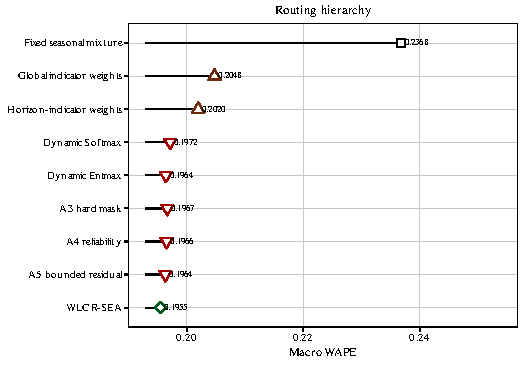
\includegraphics[width=\columnwidth]{figures/wlcr_sea_clean_accuracy.pdf}
\caption{干净留出集上的路由层级。指标专属权重解释了固定到学习改善的大部分。}
\label{fig:accuracy}
\end{figure}

\subsection{RQ2：该方法在增强匹配协议下是否保持鲁棒？}
图~\ref{fig:missingness} 的子图 (a) 展示原始模型的压力剖面，子图 (b) 和表~\ref{tab:robust-ci} 展示增强匹配的成对比较。匹配对照为 DLinear-Aug、PatchTST-Aug 和 GRU-D-Direct-Aug。

在 20\% 块缺失、20\% 时间线尾部缺失及 30\% 异步缺失时，\method{} 的 WAPE 分别为 0.2017、0.2048 和 0.2045。其相对 DLinear-Aug 和 PatchTST-Aug 的成对区间在全部六个比较中均跨越零，而上述三个 GRU-D-Direct-Aug 区间均低于零。在 50\% 请求破坏时，\method{} 在块缺失、时间线尾部缺失和异步缺失下的 WAPE 分别为 0.2196、0.2460 和 0.2172；列出的全部九个增强匹配区间均低于零。

在 50\% 破坏时，\originalmethod{} 在块/时间线尾部/异步掩码下的宏 WAPE 为 0.2636/0.3234/0.2261，而 \method{} 为 0.2196/0.2460/0.2172。该原始模型的压力剖面与增强匹配比较分开报告。

\begin{table*}[t]
\centering
\caption{成对五个种子模型集成的鲁棒性结果。表项为 \method{} 减基线的 WAPE 差异及 5,000 次未调整成对小区簇 bootstrap 95\% 区间；负值支持 \method{}。匹配基线严格为 DLinear-Aug、PatchTST-Aug 和 GRU-D-Direct-Aug；\originalmethod{} 不纳入本表。对随机机制，区间以五个固定破坏掩码实现为条件。}
\label{tab:robust-ci}
\footnotesize
\setlength{\tabcolsep}{3.0pt}
\begin{tabular}{lcccc}
\toprule
条件 & \method{} WAPE & \shortstack{$\Delta$ 相对\\DLinear-Aug [95\% CI]} & \shortstack{$\Delta$ 相对\\PatchTST-Aug [95\% CI]} & \shortstack{$\Delta$ 相对\\GRU-D-Direct-Aug [95\% CI]}\\
\midrule
20\% 块缺失 & 0.2017 & $-0.00030$ [$-0.00308$, $0.00259$] & $-0.00030$ [$-0.00379$, $0.00278$] & $-0.03339$ [$-0.04052$, $-0.02619$]\\
20\% 时间线尾部 & 0.2048 & $-0.00150$ [$-0.00407$, $0.00115$] & $-0.00168$ [$-0.00541$, $0.00182$] & $-0.05270$ [$-0.06220$, $-0.04297$]\\
30\% 异步 & 0.2045 & $-0.00175$ [$-0.00465$, $0.00124$] & $-0.00162$ [$-0.00531$, $0.00192$] & $-0.02597$ [$-0.03323$, $-0.01820$]\\
50\% 块缺失 & 0.2196 & $-0.04022$ [$-0.04562$, $-0.03500$] & $-0.02050$ [$-0.02496$, $-0.01603$] & $-0.04953$ [$-0.05590$, $-0.04317$]\\
50\% 时间线尾部 & 0.2460 & $-0.03451$ [$-0.04304$, $-0.02669$] & $-0.01569$ [$-0.02292$, $-0.00899$] & $-0.06970$ [$-0.08060$, $-0.05871$]\\
50\% 异步 & 0.2172 & $-0.02044$ [$-0.02426$, $-0.01657$] & $-0.01303$ [$-0.01701$, $-0.00913$] & $-0.03504$ [$-0.04215$, $-0.02771$]\\
\bottomrule
\end{tabular}
\end{table*}

\begin{figure*}[t]
\centering
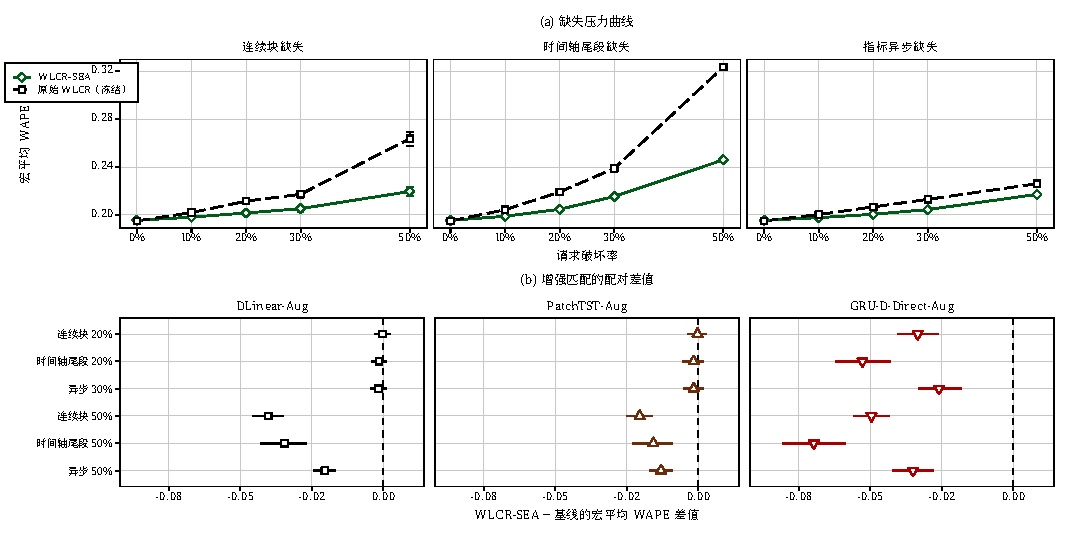
\includegraphics[width=\textwidth]{figures/wlcr_sea_missingness_zh.pdf}
\caption{缺失鲁棒性。(a) \method{} 与 \originalmethod{} 在五个固定掩码下的结果；原始模型曲线与增强匹配比较分开报告。(b) 相对增强匹配神经对照的未调整成对 95\% 区间；负值支持 \method{}。}
\label{fig:missingness}
\end{figure*}
\begin{table*}[!t]
\centering
\caption{单线程、批量为一的仅预测部署成本，包括预处理、反变换和输出下限。五成员集成采用串行执行。KiB 采用 1,024 字节，覆盖检查点与冻结模型资产，不覆盖拟议审计载荷。计时部署报告干净 WAPE。GRU-D-Direct-Aug 未纳入此 CPU 协议；“未测量”和“--”表示没有可比延迟和经审计部署资产大小，并非零成本。}
\label{tab:latency}
\footnotesize
\setlength{\tabcolsep}{4.0pt}
\begin{tabular}{llrrrrr}
\toprule
模型族 & 部署 & WAPE & P50 (ms) & P95 (ms) & P99 (ms) & KiB\\
\midrule
\method{} & 单种子（42） & 0.1959 & 6.802 & 7.301 & 7.574 & 16.2\\
\method{} & 五个种子模型集成 & 0.1955 & 34.705 & 37.420 & 38.684 & 148.8\\
DLinear-Aug & 单种子（42） & 0.1936 & \textbf{0.506} & \textbf{0.558} & \textbf{0.576} & 67.1\\
DLinear-Aug & 五个种子模型集成 & 0.1907 & 2.402 & 2.530 & 2.564 & 335.4\\
PatchTST-Aug & 单种子（42） & 0.1998 & 1.087 & 1.149 & 1.179 & 143.6\\
PatchTST-Aug & 五个种子模型集成 & 0.1960 & 7.270 & 7.482 & 7.592 & 1,057.1\\
GRU-D-Direct-Aug & 五个种子模型集成 & 0.2235 & \multicolumn{3}{c}{未测量} & --\\
\originalmethod{} & 仅话务 73 维，单种子（42） & 0.1951 & 13.290 & 14.344 & 15.425 & 9,316.8\\
\bottomrule
\end{tabular}
\end{table*}

表~\ref{tab:variants} 区分 A3--A6 机制。其干净 WAPE 分别为 0.1967、0.1966、0.1964 和 0.1955。在从 A1--A3 的每条输入和损失路径中移除可靠性后，A4 与 A3 的点差仍然很小。因此，可靠性主要作为可审计的支撑描述符；有界残差带来很小的干净点估计改善，而主要的严重缺失优势与混合增强相关。

\subsection{RQ3：哪些审计主张经得起直接测试？}
结构检查均严格通过。跨五个模型种子，不可用专家的最大权重为 0，所有有界包络检查的最大违例均为零。有效支持集平均包含 $5.223$ 个专家；五个独立训练成员给出 $[5.101,5.345]$ 的 95\% 种子层 $t$ 区间。因此，此处稀疏性意味着严格零值，而非单专家路由。相对于基线，残差在多数预测中仍很小：五个种子模型的平均 P50/P90 比例为 0.00615/0.03068。

实现层局部性测试在 253 个小区、全部七个评估日期和四个缺失分箱上确定性地分层抽取 256 个目标请求。对每个目标，在保留目标对象的同时，扰动每个非目标预提取请求对象（包括同小区非目标对象）。在全部 256 次测试中，专家值、掩码、可靠性、上下文、注意力、基线、残差、熵和预测均按位一致（$N_{\mathrm{violations}}=0$）。这在记录的字段白名单下建立了服务路径的请求对象级不变性。

删除效果通过重新计算获得，而非通过缓存权重重新归一化近似：对选定的可用非先验专家施加硬掩码，将其可靠性置零，并重新运行注意力与残差。在五个种子模型集成中，删除最高权重专家使宏 WAPE 增加 0.00595（小区簇 bootstrap CI $[0.00441,0.00757]$），而期望匹配的随机删除为 0.00104（$[0.00079,0.00131]$；每个模型种子重复 10 次）。在五个成员模型上，专家权重与留一预测影响之间的逐成员 Spearman 相关平均为 0.693（95\% 种子层 $t$ 区间 $[0.678,0.708]$）。这些删除结果在所记录审计范围内支持行为相关性。

相较之下，五个成员的熵--APE Spearman 相关均值为 $-0.0196$（95\% 种子层 $t$ 区间 $[-0.0407,0.0016]$），因此注意力熵不被用作不确定性估计。图~\ref{fig:audit} 汇总了这些发现。

\begin{figure*}[t]
\centering
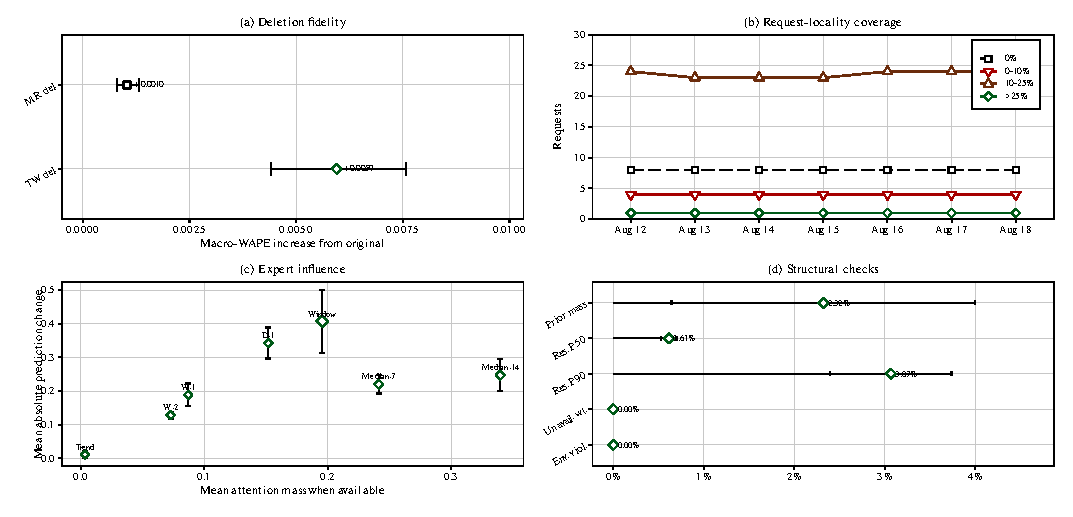
\includegraphics[width=\textwidth]{figures/wlcr_sea_auditability.pdf}
\caption{可审计性证据：重路由删除、专家影响、结构检查，以及覆盖 256 个请求的零违例局部性。图中轴标签简写：TW/最高权重，MR/匹配随机，del./“删”=删除，Res.=残差，wt.=权重，Unavail./“不可用”=不可用专家，Env./“包络违例”=有界包络违例，Prior mass/“先验权重”=平均先验权重。}
\label{fig:audit}
\end{figure*}
\subsection{RQ4：小区不相交重拟合下观察到何种表现，其部署成本如何？}
五个确定性小区不相交折将评估小区排除在每个折拟合量之外，并以零小区重叠覆盖全部 \RQFourEvaluationWindowCount{} 个窗口。在协议匹配的单模型种子（\RQFourModelSeed{}）重拟合下，\method{} 的 WAPE 为 \RQFourWLCRWAPE{}，DLinear-Aug 为 \RQFourDLinearWAPE{}；二者成对差异为 $\RQFourDLinearDelta{}$，未调整的 95\% 小区簇 bootstrap 区间为 $[\RQFourDLinearCILow{},\RQFourDLinearCIHigh{}]$。相对 \originalmethod{}（\RQFourOriginalWAPE{}），差异为 $\RQFourOriginalDelta{}$，区间为 $[\RQFourOriginalCILow{},\RQFourOriginalCIHigh{}]$；相对 PatchTST-Aug（\RQFourPatchWAPE{}），差异为 $\RQFourPatchDelta{}$，区间为 $[\RQFourPatchCILow{},\RQFourPatchCIHigh{}]$。同小时中位数和 \fixedmixture{} 的点 WAPE 分别为 \RQFourSameHourWAPE{} 和 \RQFourFixedMixtureWAPE{}。这些描述性区间重采样 \RQFourClusterCount{} 个小区，并以固定的种子 \RQFourModelSeed{} 重拟合为条件；它们不量化优化种子或协议选择不确定性。各折未见小区的平均先验权重为 \RQFourPriorMassPercent{}\%。

表~\ref{tab:latency} 将每个计时的仅预测部署与其自身干净 WAPE 配对。主要精度结果采用五个种子模型集成，因此其 34.70/38.68 ms 的 P50/P99 延迟及 148.8 KiB 的检查点和冻结模型资产是与部署对齐的值。五个成员在同一单线程设置上串行执行，并为每个成员重新计算预处理。该表报告从请求局部预处理到反变换和输出下限的仅预测推理。DLinear 和 PatchTST 仍更快，而仅话务 \originalmethod{} 比单个 \method{} 成员更大且更慢。



\section{讨论}\label{sec:discussion}
专家库由人工指定，偏向周期性行为；没有局部先例的突发事件可能被遗漏。Entmax 会产生严格零值，但多数预测仍使用约五个专家。经校正的消融中，可靠性描述符没有独立性能证据；无增强时，有界残差可能损害鲁棒性。这些模块不应被表述为同等的增益来源。

当前轨迹覆盖一个匿名区域和约一个月。全部起点均为午夜，故预测步长与时钟小时混杂；需要更多起点、季节和区域才能评估外部泛化。8 月留出集曾用于重设计，故当前评估仍属探索性，有待在此前未用于研究的前瞻性时间段上验证。小区不相交分析是同一轨迹内的排除审计，而非跨区域泛化证据。它固定一个模型种子（42），使用一个匹配的确定性最终重拟合增强视图，且不进行折特异或嵌套再调优。其小区簇 bootstrap 区间在固定这些重拟合的条件下重采样 727 个观测小区，因此不包含重新训练、超参数选择、时间或区域不确定性。因此，区间低于零仅表示所记录比较中的方向性结果，并非模型族层面的普遍优势证据。

GRU-D-Direct-Aug 提供专用的缺失感知直接预测对照，原始模型的压力剖面与增强匹配比较分开报告。成对区间是未调整的描述性估计，并以五个固定破坏掩码实现为条件；它刻画跨小区不确定性，而非跨模型族、机制、缺失率、指标和审计测试的族层效应。破坏机制保持跨请求的绝对时间线一致性。五个种子模型集成提高报告精度，但也使服务成本成倍增加；表~\ref{tab:latency} 同时报告集成和单成员部署。

请求对象服务路径不变性在记录的字段白名单下被验证为一项实现属性；上游请求构造不在本测试范围内。该服务路径并非隐私保证，因为全局参数和冻结先验编码训练分布信息。注意力和删除分析刻画行为相关性，而熵不提供有用的不确定性估计。未来扩展可在评分路径可用时纳入天气、坐标、静态参数、资源配置和运行调度信息。

服务策略刻画了一条自包含的在线评分路径。后续研究可量化入口与评分分离的可用性、延迟和故障隔离属性，并将该接口与使用获授权邻居状态的图模型进行比较。这类评估将刻画请求局部证据与更丰富的空间证据发挥互补价值的条件。

\section{结论}
结构化季节专家路由将固定请求局部混合转化为预测步长条件化、可用集合掩码和有界的预测路径，并提供拟议固定模式语义审计记录的核心字段。在干净历史上，\method{} 相对 \originalmethod{} 的未调整成对区间包含零，因此该分析未检测到差异；DLinear 的干净 WAPE 最低。在匹配增强下，相对 DLinear-Aug 和 PatchTST-Aug 的选定中等缺失比较区间包含零；而在列出的 50\% 结构化破坏条件下，相对三个增强匹配基线的九个差异均为负且区间均低于零，这些结果以五个固定掩码为条件。记录的实现检查得到不可用专家权重为零、有界包络违例为零，并在字段白名单下的 256 个分层请求对象测试中保持按位一致的服务路径不变性。在协议匹配的单种子小区不相交重拟合下，相对 DLinear-Aug 和 \originalmethod{} 的区间包含零，而相对 PatchTST-Aug 的区间低于零。由于这些区间以固定重拟合为条件，它们不能建立重新训练或跨区域泛化结论。因此，现有证据识别出面向请求局部服务的探索性鲁棒性--可检查性--成本剖面。仍需在更长、跨区域和跨季节数据上开展前瞻验证，并与使用获授权邻居信息的方法比较，才能判断该剖面如何泛化。

\section*{代码与数据获取}
实现代码已在
\url{https://github.com/rudykon/WLCR-SEA_Predictor}
开源。数据获取的相关说明亦可参见该链接。

\bibliographystyle{IEEEtran}
\bibliography{references}

\end{document}
